\documentclass[12pt,letterpaper]{article}
\usepackage{fullpage}
\usepackage[top=2cm, bottom=4.5cm, left=2.5cm, right=2.5cm]{geometry}
\usepackage{amsmath,amsthm,amsfonts,amssymb,amscd}
\usepackage{lastpage}
\usepackage{enumerate}
\usepackage{fancyhdr}
\usepackage{mathrsfs}
\usepackage{xcolor}
\usepackage{graphicx}
\usepackage{listings}
\usepackage{hyperref}
\usepackage{tikz}

\hypersetup{%
  colorlinks=true,
  linkcolor=blue,
  linkbordercolor={0 0 1}
}

\renewcommand\lstlistingname{Algorithm}
\renewcommand\lstlistlistingname{Algorithms}
%\def\lstlistingautorefname{Alg.}

\lstdefinestyle{Python}{
    language        = Python,
    %frame           = lines,
    basicstyle      = \footnotesize,
    keywordstyle    = \color{blue},
    stringstyle     = \color{green},
    commentstyle    = \color{red}\ttfamily
}

\setlength{\parindent}{0.0in}
\setlength{\parskip}{0.05in}

% Edit these as appropriate
\newcommand\course{CSCI 5352}
\newcommand\psnumber{3}                  % <-- homework number
\newcommand\name{Cassandra Spath}
\newcommand\duedate{October 9, 2019}

\pagestyle{fancyplain}
\headheight 35pt
\lhead{\name}
\chead{\textbf{\Large Problem Set \psnumber}}
\rhead{\course \\ \duedate}
\lfoot{}
\cfoot{}
\rfoot{\small\thepage}
\headsep 1.5em

\begin{document}

\begin{enumerate}
\itemsep1em

    \item  (15 pts) Assuming the couples interviewed to be a representative sample of the edges in the undirected network of relationships for the community studied, and treating the vertices as being of four types—black, hispanic, white, and other—calculate the numbers $e_{rr}$ and $a_r$ that appear in Eq. (7.76) in Networks for each type. Hence calculate the modularity $Q$ of the network with respect to ethnicity. What do you conclude about homophily in this community?

    \begin{align*}
        & \qquad e_{bb} = 0.258 \qquad e_{hh} = 0.157 \qquad e_{ww} = 0.306 \qquad e_{oo} = 0.016 \\
        & \qquad a_b^2 = a_{bM}*a_{bW} = 0.322*0.288 \qquad  a_h^2 = 0.246*0.203 \\
        & \qquad a_w^2 = 0.377*0.423 \qquad a_o^2 = 0.052*0.083 \\ \\
        Q &= \sum_{r} (e_{rr} - a_r^2) \\
        &= e_{bb} - a_b^2 + e_{hh} - a_h^2 + e_{ww} - a_w^2 + e_{oo} - a_o^2 \\
        &= 0.258 - (0.322*0.288) + 0.157 - (0.246*0.203) + 0.306 - (0.377*0.423) + \\& \qquad 0.016 - (0.052*0.083) \\
        &= 0.4305
    \end{align*}

    \newpage
    \item (20 pts total) Consider an undirected “line graph” consisting of $n$ vertices in a single component, with diameter $n - 1$, and composed of $n - 2$ vertices with degree 2 and 2 vertices with degree 1.
    \begin{enumerate}
    \itemsep1em
        \item Show mathematically that if we divide this network into any two contiguous groups, such that one group has $r$ connected vertices and the other has $n - r$, the modularity $Q$ takes the value
        $$Q = \frac{3 - 4n + 4rn - 4r^{2}}{2(n - 1)^2}$$

        The $r$ vertices will have $r-1$ edges between them. There is $1$ edge between the two groups. The $n-r$ vertices have $n-r-1$ edges between the them. This allows the calculation of $e_{rr}$ and $a_r$ values which are then used to calculate the modularity $Q$.

        \begin{center}
            \begin{tabular}{c|c|c||c}
                [e] & r & n-r & a \\
                \hline
                \hline
                r & $\frac{r-1}{n-1}$ & $\frac{1}{2(n-1)}$ & $\frac{2r-1}{2(n-1)}$ \\
                \hline
                n-r & $\frac{1}{2(n-1)}$ & $\frac{n-r-1}{n-1}$ & $\frac{2n-2r-1}{2(n-1)}$
            \end{tabular}
        \end{center}

        \begin{align*}
            Q &= \sum_{r} (e_{rr} - a_r^2) \\
            &= \frac{r-1}{n-1} - \left(\frac{2r-1}{2(n-1)}\right)^2 + \frac{n-r-1}{n-1} - \left(\frac{2n-2r-1}{2(n-1)}\right)^2 \\
            &= \frac{4(r-1)(n-1)-(2r-1)^2+4(n-r-1)-(2n-2r-1)^2}{4(n-1)^2} \\
            &= \frac{4(n-1)(r-1+n-r-1) - (4r^2 -4r +1) - (4n^2 - 4n - 8rn + 4r^2 + 4r + 1)}{4(n-1)^2} \\
            &= \frac{4n^2-12n+8 -8r^2 + 8rn + 4n -2}{4(n-1)^2} \\
            &= \frac{6-8n -8r^2 + 8rn}{4(n-1)^2} \\
            &= \frac{3 -4n -4r^2 + 4rn}{2(n-1)^2} \\
        \end{align*}

        \newpage
        \item Considering the same graph, show that when n is even, the optimal division, in terms of modularity $Q$, is the division that splits the network exactly down the middle, into two parts of equal size.

        Assume $n$ is even and the network is split in half. Then, $r = n/2$.
        \begin{align*}
            Q &= \frac{3 - 4n + 4rn - 4r^{2}}{2(n - 1)^2} \\
            &= \frac{3 - 4n + 4 (\frac{n}{2})n - 4 (\frac{n}{2})^2} {2(n-1)^2} \\
            &= \frac{3 - 4n + 2 n^2 - n^2} {2(n-1)^2} \\
            &= \frac{3 - 4n + n^2} {2(n-1)^2}
         \end{align*}

         Assume $n$ is even and the network is not split in half. Then $r = \frac{n}{2} -x$ for some integer x such that $0 < x < n/2$.
        \begin{align*}
            Q =& \frac{3 - 4n + 4rn - 4r^{2}}{2(n - 1)^2} \\
            =& \frac{3 - 4n + 4 (\frac{n}{2}-x)n - 4 (\frac{n}{2}-x)^2} {2(n-1)^2} \\
            =& \frac{3 - 4n + 2 n^2 - 4nx - n^2 +4x^2} {2(n-1)^2} \\
            =& \frac{3 - 4n + n^2 -4nx +4x^2} {2(n-1)^2}
        \end{align*}
        The difference between the two Q values is
        $$ \frac{3 - 4n + n^2 -4nx +4x^2} {2(n-1)^2} - \frac{3 - 4n + n^2} {2(n-1)^2} = -4nx +4x^2 $$

        Since $1 \leq x \leq \frac{n}{2}$, the difference would be negative for any valid value of x. Thus, having any division of the network that isn't in half would result in a smaller modularity than the optimal split of half the nodes in each group.

    \end{enumerate}

    \newpage
    \item (30 pts) Implement the greedy agglomerative algorithm described in the lecture notes for maximizing modularity on an unlabeled simple network. (There is no need to make your algorithm particularly efficient, as we will not apply it to large networks; thus, it is okay to compute $\Delta Q$ using the adjacency matrix to derive the $e$ matrix at each step.)

    \begin{itemize}
        \item Make a plot showing the modularity score $Q$ as a function of the number of merges.

        \item Make a visualization of the network itself with vertices labeled according to your maximum modularity partition.

        \item Then calculate and report the normalized mutual information (NMI) between your partition and the social partition.

        \item Finally, briefly discuss the agreement or disagreement between the two partitions, and what that agreement/disagreement implies about the utility of modularity maximization inferring good partitions without knowing such labels.

    \end{itemize}

    \begin{figure}[!h]
        \centering
        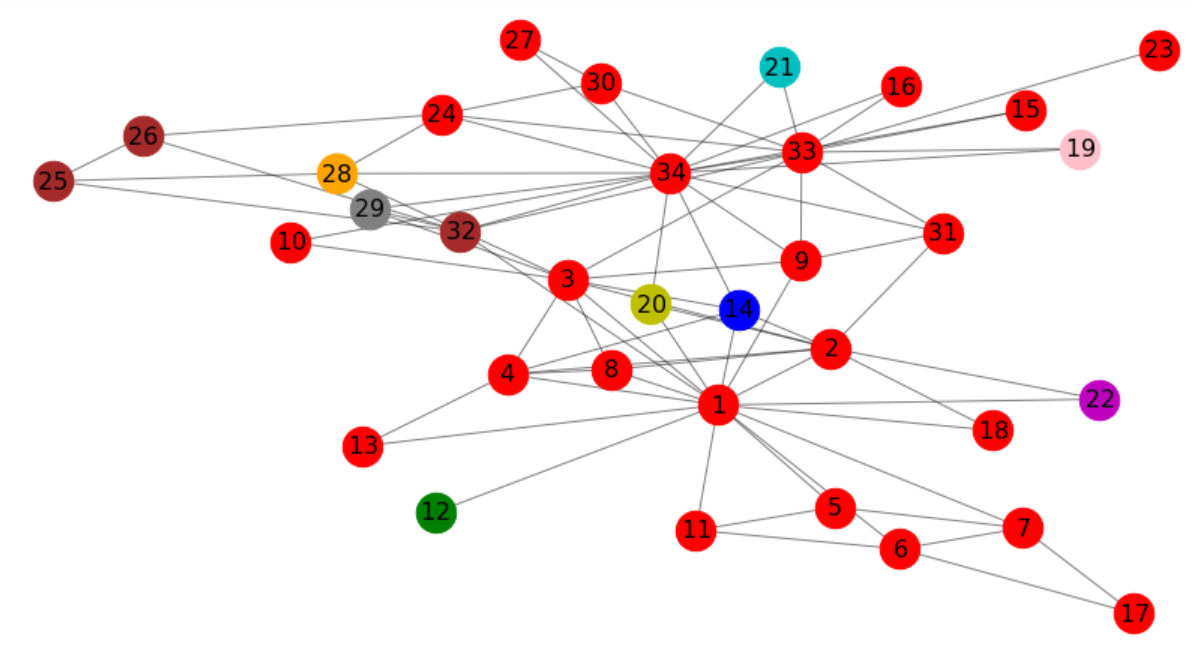
\includegraphics[width=1\linewidth]{ps3-3b.png}
    \end{figure}


    \begin{figure}[!h]
        \centering
        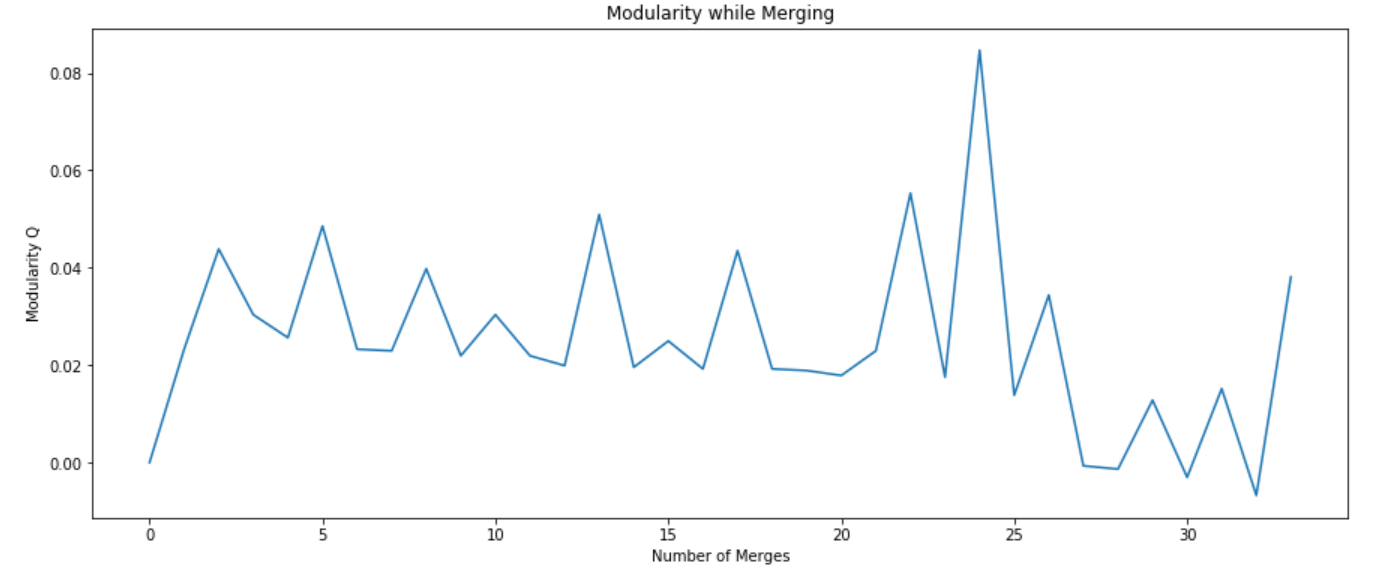
\includegraphics[width=1\linewidth]{ps3-3.png}
    \end{figure}

    The normalized mutual information (MNI) between the partitions is 0.2415.

    Given the MNI value, the two partitions do not agree. Thus, modularity maximization without knowing labels does not result in the best partitions of the data. Since this is purely a maximum and the accurate partitions aren't necessarily a maximum.

    \newpage
    \item  (35 pts) Using the FB100 networks, investigate the assortativity patterns for three vertex attributes: (i) student/faculty status, (ii) major, and (iii) vertex degree. Treat these networks as simple graphs in your analysis.

    For each vertex attribute, make a scatter plot showing the assortativity versus network size $n$, on log-linear axes, for all 100 networks, and a histogram or density plot showing the distribution of assortativity values. In both figures, include a line indicating no assortativity. Briefly discuss the degree to which vertices do or do not exhibit assortative mixing on each attribute, and speculate about what kind of processes or tendencies in the formation of Facebook friendships might produce this kind of pattern.

    \begin{figure}[!h]
        \centering
        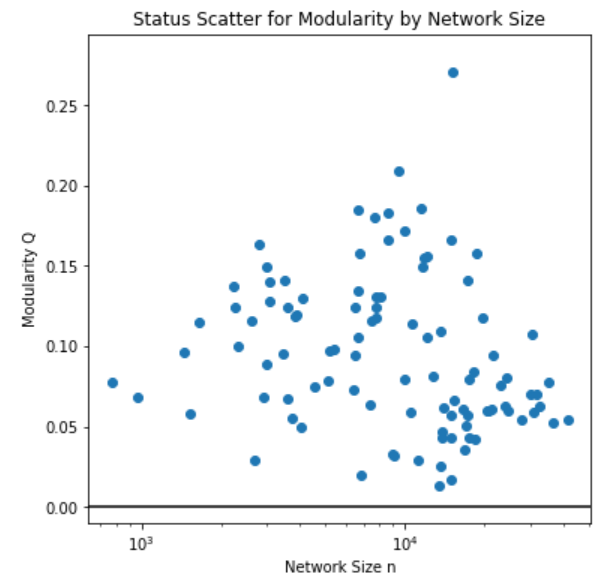
\includegraphics[width=0.5\linewidth]{ps3-4status1.PNG}
        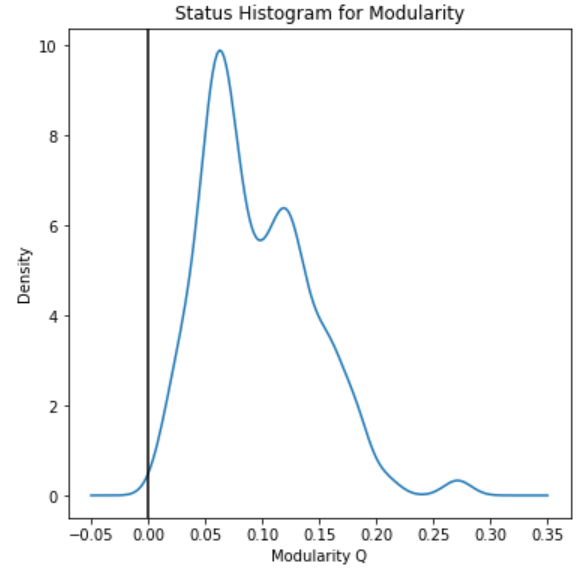
\includegraphics[width=0.5\linewidth]{ps3-4status2.PNG}
    \end{figure}

    For the status of the nodes, there is a clear assortivity between the nodes. The nodes mostly connect to those with the same status. Since the modularity values are somewhat large, there are few edges between nodes of different groups. There is homophily by status.

    \begin{figure}[!h]
        \centering
        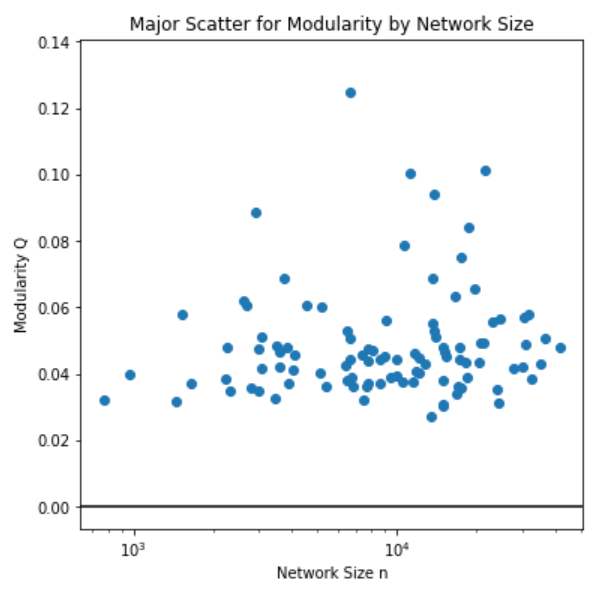
\includegraphics[width=0.5\linewidth]{ps3-4major1.PNG}
        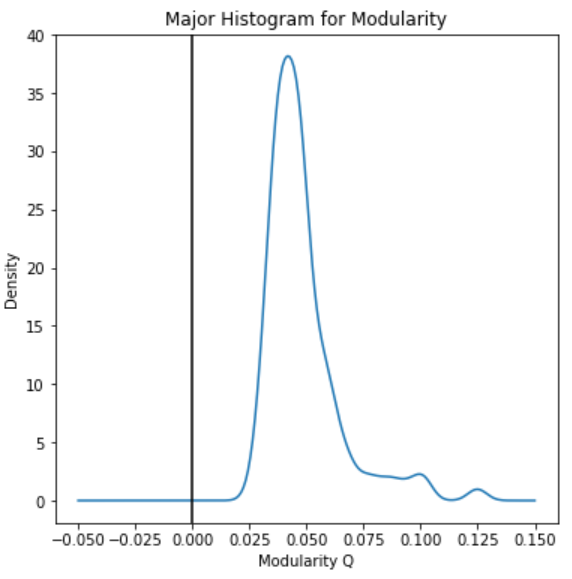
\includegraphics[width=0.5\linewidth]{ps3-4major2.PNG}
    \end{figure}

    For the major of the nodes, there is assortivity between the nodes. Nodes connect with those of the same major. The modularities are large so there are few connections between groups. Most connections exist between nodes of the same group. This suggest homophily by major.

    \begin{figure}[!h]
        \centering
        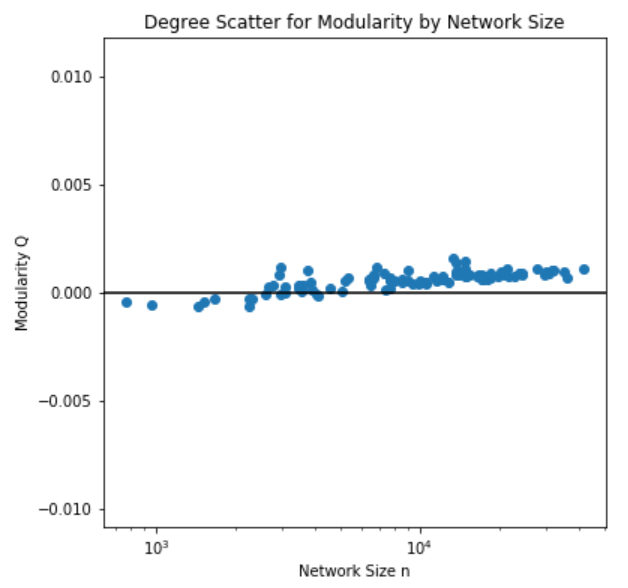
\includegraphics[width=0.5\linewidth]{ps3-4degree1.PNG}
        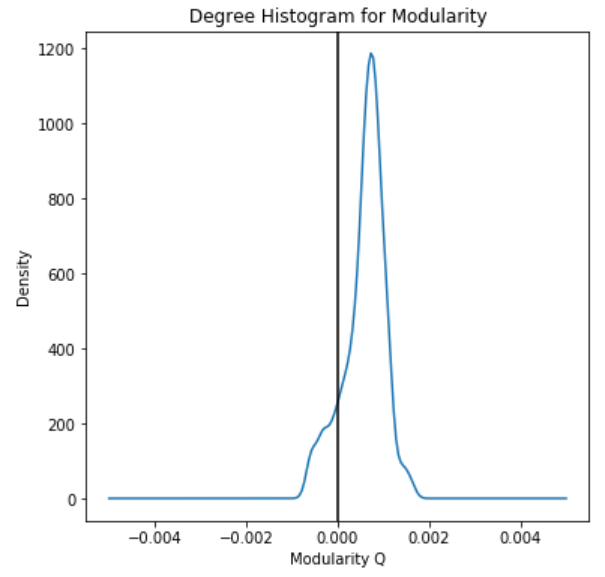
\includegraphics[width=0.5\linewidth]{ps3-4degree2.PNG}
    \end{figure}

    The degree of the node has a small amout of assortivity. Nodes with higher degrees tend to connect to other nodes with higher degrees. However, the modularity is still very small meaning that this doesn't have a huge effect. Thus this is homophily by degree but has a small impact.

    \newpage
    \item (10 pts extra credit) As described in Section 13.2 of Networks, the configuration model can be thought of as the ensemble of all possible matchings of edge stubs, where vertex $i$ has $k_i$ stubs. Show that for a given degree sequence, the number $\Omega$ of matchings is
    $$\Omega = \frac{(2m)!}{2^m m!}$$
    which is independent of the degree sequence.

    \item  (15 pts extra credit) Using the configuration model, investigate the set of random graphs in which all vertices have degree 1 or 3.

    \begin{itemize}
        \item Calculate via computer simulation the mean fractional size of the largest component for a network with $n = 10^4$ vertices, and with $p_1 = 0.6$, $p_3 = 1 − p_1$, and $p_k = 0$ for all other values of $k$.

        \item Now make a figure showing the mean fractional size of the largest component for values of $p_1$ from 0 to 1 in steps of 0.01. Show that this allows you to estimate the value of $p_1$ for the phase transition at which the giant component disappears.

        \item Do your results depend on which graph space you choose for your configuration model?
    \end{itemize}
\end{enumerate}

\newpage
\lstset{caption={Python Code for Problems 3 and 4}}
\begin{lstlisting}[style = Python]
import numpy as np
import matplotlib.pyplot as plt
import os
import networkx as nx
from scipy.stats import gaussian_kde
from sklearn.metrics.cluster import normalized_mutual_info_score

#PROBLEM 3
#agglomeration algo
def greedyAgglomeration(A, groups, m):
    # separate the nodes into their own groups and 0 as the first delta Q
    if not groups:
        groups = []
        for i in range(len(A)):
            groups.append([i])
        q = [0]
        q.extend(greedyAgglomeration(A, groups, m))
        return q
    # if all the nodes are in one group, return an empty array
    if len(groups) == 1:
        return []
    # maximum change in delta Q and indices of groups
    maxDeltaQ = -10**10
    indices = (-1,-1)
    # loop through pairs of groups
    for i in range(len(groups)):
        for j in range(i+1,len(groups)):
            # calculate av, au, and e for the two group
            e = 0
            av = 0
            for v in groups[i]:
                av += np.sum(A[v])
                au = 0
                for u in groups[j]:
                    e += A[v][u]
                    au = np.sum(A[u])
            e /= m
            # calculate the delta Q for the two groups, choose maximum
            deltaQ = 2*(e - (av/m)*(au/m))
            if maxDeltaQ < deltaQ:
                maxDeltaQ = deltaQ
                indices = (i, j)
    # combine the two groups from the maximum delta Q
    groups[indices[0]].extend(groups[indices[1]])
    groups.pop(indices[1])
    # extend the maximum delta Q by the recursive array of values and return
    q = [maxDeltaQ]
    q.extend(greedyAgglomeration(A, groups, m))
    return q

n = 34
A = np.array([[0 for i in range(n)] for j in range(n)])
edges = []
with open("karate_edges_77.txt", "r") as f:
    data = f.readline()
    while data:
        vals = data.split("\n")[0].split("\t")
        A[int(vals[0])-1][int(vals[1])-1] = 1
        edges.append((int(vals[0])-1,int(vals[1])-1))
        data = f.readline()
f.close()
m = np.sum(A)/2

G = nx.Graph()
G.add_edges_from(edges)

(deltaQ, groups) = greedyAgglomeration(A, None, m)
fig, ax = plt.subplots(figsize=(15, 6))
ax.plot(range(0,len(deltaQ)), deltaQ)
ax.set_ylabel("Modularity Q")
ax.set_xlabel("Number of Merges")
ax.set_title("Modularity while Merging")
plt.show()

pos=nx.spring_layout(G) # positions for all nodes
fig, ax = plt.subplots(figsize=(15, 8))

colors = ['r','g','b','#FFC0CB','y','c','m','#A52A2A','#FFA500','#808080']
for (group,color) in zip(groups,colors):
  nx.draw_networkx_nodes(G,pos,
                          nodelist=group,
                          node_color=color,
                          node_size=700)
nx.draw_networkx_edges(G,pos,width=1.0,alpha=0.5)

labels={}
for i in range(0,n):
  labels[i]=r'$'+str(i+1)+'$'
  nx.draw_networkx_labels(G,pos,labels,font_size=16)

ax.axis('off')
plt.show()

labels = [0 for i in range(n)]
j = 0
for group in groups:
    for i in group:
        labels[i] = j
    j += 1
social_labels = [0,0,0,0,0,0,0,0,0,1,0,0,0,0,1,1,0,0,1,0,1,0,1,1,1,1,1,1,1,1,1,1,1,1]
print(len(social_labels))
normalized_mutual_info_score(labels, social_labels, average_method='warn')

#PROBLEM 4
def calcModularity(A, x, numTypes):
    n = len(A)
    m = np.sum(np.sum(A))
    # calculate e matrix
    e = [[0 for i in range(numTypes)] for j in range(numTypes)]
    for i in range(n):
        for j in range(n):
            if A[i][j]:
                u = x[i]
                v = x[j]
                e[u][v] += 1
    e = e / m
    # calculate a array
    a = np.sum(e, axis=1)
    # calculate modularity Q
    Q = 0
    for u in range(numTypes):
        Q += (e[u][u] - a[u]*a[u])
    return Q

directory = "facebook100txt"
modStatus = []
modMajor = []
modDegree = []
networkSize = []
for filename in os.listdir(directory):
    if not filename.endswith("_attr.txt"):
        node_list_status = []
        node_list_major = []
        with open(directory+"/"+filename.split(".txt")[0]+"_attr.txt", "r") as f:
            data = f.readline()
            data = f.readline()
            while data:
                vals = data.split("\n")[0].split("\t")
                node_list_status.append(int(vals[0]))
                node_list_major.append(int(vals[2]))
                data = f.readline()
        f.close()

        n = len(node_list_status)
        A = np.array([[0 for i in range(n)] for j in range(n)])
        with open(directory+"/"+filename, "r") as f:
            data = f.readline()
            while data:
                vals = data.split("\n")[0].split("\t")
                A[int(vals[0])-1][int(vals[1])-1] = 1
                data = f.readline()
        f.close()

        networkSize.append(n)
        node_list_degree = np.sum(A, axis=1)

        modStatus.append(calcModularity(A,node_list_status,np.max(node_list_status)+1))
        modMajor.append(calcModularity(A,node_list_major,np.max(node_list_major)+1))
        modDegree.append(calcModularity(A,node_list_degree,np.max(node_list_degree)+1))

# scatter status
ax.scatter(networkSize, modStatus)
ax.set_ylabel("Modularity Q")
ax.set_xlabel("Network Size n")
ax.set_title("Status Scatter for Modularity by Network Size")
ax.set_xscale("log")
ax.axhline(0, color="k")

# histogram status
density = gaussian_kde(modStatus)
xs = np.linspace(-0.05,0.35,200)
density.covariance_factor = lambda : .25
density._compute_covariance()
fig, ax = plt.subplots(figsize=(15, 8))
ax.plot(xs,density(xs))
ax.set_ylabel("Density")
ax.set_xlabel("Modularity Q")
ax.set_title("Status Histogram for Modularity")
ax.axvline(0, color="k")

# scatter major
fig, ax = plt.subplots(figsize=(15, 8))
ax.scatter(networkSize, modMajor)
ax.set_ylabel("Modularity Q")
ax.set_xlabel("Network Size n")
ax.set_title("Major Scatter for Modularity by Network Size")
ax.set_xscale("log")
ax.axhline(0, color="k")

# histo major
density = gaussian_kde(modMajor)
xs = np.linspace(-0.05,0.15,200)
density.covariance_factor = lambda : .25
density._compute_covariance()
fig, ax = plt.subplots(figsize=(15, 8))
ax.plot(xs,density(xs))
ax.set_ylabel("Density")
ax.set_xlabel("Modularity Q")
ax.set_title("Major Histogram for Modularity")
ax.axvline(0, color="k")

# scatter degree
fig, ax = plt.subplots(figsize=(15, 8))
ax.scatter(networkSize, modDegree)
ax.set_ylabel("Modularity Q")
ax.set_xlabel("Network Size n")
ax.set_title("Degree Scatter for Modularity by Network Size")
ax.set_xscale("log")
ax.axhline(0, color="k")

# histo degree
density = gaussian_kde(modDegree)
xs = np.linspace(-0.005,0.005,200)
density.covariance_factor = lambda : .25
density._compute_covariance()
fig, ax = plt.subplots(figsize=(15, 8))
ax.plot(xs,density(xs))
ax.set_ylabel("Density")
ax.set_xlabel("Modularity Q")
ax.set_title("Degree Histogram for Modularity")
ax.axvline(0, color="k")
\end{lstlisting}

\end{document}
